\chapter{User Manual}
\label{usermanual}

\section{ESP32 System Setup}\label{sec:SysSetupESP32}
In this Section, the set of both hardware and software resources required to set up the ESP32 are outlined. 
At the end of this Section, you will have acquired a clear overview of the
prerequisites to set up the environment and run a project. It is strongly recommended to use a virtual machine (use Virtual Box\cite{virtualbox}) 
or machine with a Linux distribution (i.e. Ubuntu Linux\cite{Ubuntu}) installed as operating system and to follow this guide to set up everything.

\subsection{Hardware resources}

\begin{itemize}
  \item \textbf{ESP32 board}.
  \item \textbf{USB cable} - USB A /micro USB B
  \item \textbf{Computer} running Windows, Linux, or macOS
\end{itemize}

This document will focus only on the implementation for the Linux environment. In case of using a virtual machine, 
make sure that the USB ports are visible to your system and internet connection is provided by WiFi bridge (take a look in Known Issues \ref{sec:problems}).

\subsection{Software resources}
You need the following tools:

\begin{itemize}
  \item \textbf{Toolchain} to compile code for ESP32
  \item \textbf{Build tools} - Cmake and Ninja to build a full Application for ESP32
  \item \textbf{ESP-IDF} that essentially contains API (software libraries and source code) for ESP32 and scripts to operate the Toolchain
  \item \textbf{IDE} for C language, on your choice, to edit better the code (OPTIONAL, not covered in this report) 
\end{itemize}

\section{Guide for Linux}
This section provides a summary on getting everything installed and ready to use on Linux (Ubuntu or Debian).
All the reported material is based on the official guide provided by Espressif\cite{Espressif} end various trials.\\
\\\textbf{NOTE}: Install process of Oracle VirtualBox VM and a Linux distribution on it, is not reported in this paper. 

\subsection{Step 1 - Install Prerequisites}
In order to use ESP-IDF with the ESP32, some software packages need to be installed.
Open a terminal and run the following command:

\begin{lstlisting}
sudo apt-get install git wget flex bison gperf python3 python3-venv pip
cmake ninja-build ccache libffi-dev libssl-dev dfu-util libusb-1.0-0
\end{lstlisting}

\subsection{Step 2 - Get ESP-IDF}
To build applications for the ESP32, software libraries provided by Espressif are needed.
\\Download it from here \cite*[\href{https://github.com/espressif/esp-idf.git}{ESP-IDF}]{Git_ESP}
\\Or open a Terminal, and run the following commands:

\begin{lstlisting}
mkdir -p ~/esp
cd ~/esp
git clone -b v4.4.1 --recursive 
    https://github.com/espressif/esp-idf.git esp-idf-v4.4.1
\end{lstlisting}

\textbf{NOTE}: Is strongly recommended to use the ESP-IDF v4.4.1
\subsection{Step 3 - Set up the tools}
Aside from the ESP-IDF, you also need to install the tools used by ESP-IDF, such as the compiler, debugger, Python packages, etc, for projects supporting ESP32.

\begin{lstlisting}
cd ~/esp/esp-idf-v4.4.1
./install.sh ESP32
\end{lstlisting}

\subsection{Step 4 - Set up the environment variables}\label{sec:envSetup}
This step \textbf{must} be executed every time a new Terminal is opened in order to build, flash, etc.
\\In the terminal where ESP-IDF is going to be used, run:

\begin{lstlisting}
. $HOME/esp/esp-idf-v4.4.1/export.sh
\end{lstlisting}

\section{Start the TCP/IP WG project on ESP32}\label{sec:WGprog}
This project is located in the \textbf{ESP32\_tcpprompt\_wg} directory.

Before continue in this section is recommended to set up the Wireguard server, a small guide is provided in section \ref{sec:server} of the Appendix. 
Is strongly recommended to use a Linux Machine or an Android device as a Server. 
Remember to generate the Keys, see in section \ref{sec:server}
This is because for the simple TCP/IP communication built for this project, Netcat is needed to listen on a specific port and it is only available for Linux and Android.
Here are reported the Crypto key Routing Tables WireGuard network interface on both client and server side.

\textbf{Server}:
\begin{lstlisting}
[Interface]
Address = 192.168.77.1/24  # Network Interface IP addr. of the Server
ListenPort = 51820  # default Listening port for UDP communication
PrivateKey = GIqk1aeXqvV1WK6P8+1tplf7JDSUvl46sh02cVHPY2A=  # sK Server 

[Peer]
PublicKey = avs2h9rnmboc0o95q/zFEVOa3fFxVNqhW5kE83Zksm4=  # pK Client
AllowedIPs = 192.168.77.2/32  # Network Interface IP addr. of the Client
\end{lstlisting}

\textbf{Client}:
\begin{lstlisting}
[Interface]
Address = 192.168.77.2  # Network Interface IP addr. of the Client
ListenPort = 51820  # default Listening port for UDP communication
PrivateKey = qEnqWM2tORDVhvTZeGlK+c5jGxiFeVBRLiFPx8iAtXg=  # sK Client 

[Peer]
PublicKey = dk0lTzfwjmWHtggRkw8rmUkQQqox26G8QSBAdXebAwQ=  # pK Server
AllowedIPs = 0.0.0.0  # So that all traffic goes through the tunnel
\end{lstlisting}

The IP Addresses of the Network interfaces 192.168.77.1 for the Server and 192.168.77.2 for the client 
were chosen a priori, any other available IP Address can be used. The Private and Public keys of each Peer were generated using the code provided in this section \ref{sec:server}.

\textbf{NOTE:} On the client side, so on the ESP32 in this case, also the \textbf{Endpoint} must be configured. During the tests 
the router assigned to the ESP32 the IP Address:'192.168.43.131'. In this case Endpoint: '\textbf{192.168.43.131:51820}'

\subsection{Configure the Project}
Remember to set the environment variable \ref{sec:envSetup} if not done.
Copy the project \texttt{/ESP32\_tcpprompt\_wg}  to \texttt{\textasciitilde /esp} directory:

\begin{lstlisting}
cd ~/esp
cp -r $IDF_PATH/ESP32_tcpprompt_wg .
\end{lstlisting}

Here there should be \texttt{esp-idf} and \texttt{ESP32\_tcpprompt\_wg} folders in the same directory.
Navigate to the project directory, set ESP32 as the target (To do only the first time), and run the project configuration utility menuconfig in order to set up your configuration.

\begin{lstlisting}
cd ~/esp/ESP32_tcpprompt_wg
idf.py set-target ESP32
idf.py menuconfig
\end{lstlisting}

After the \texttt{idf.py menuconfig} command, the following window should appear \ref{fig:menuConfig}.
In this window many basic parameters of the ESP32 can be set.

\begin{figure}[H]
    \vspace{0.4cm}
    \centering
    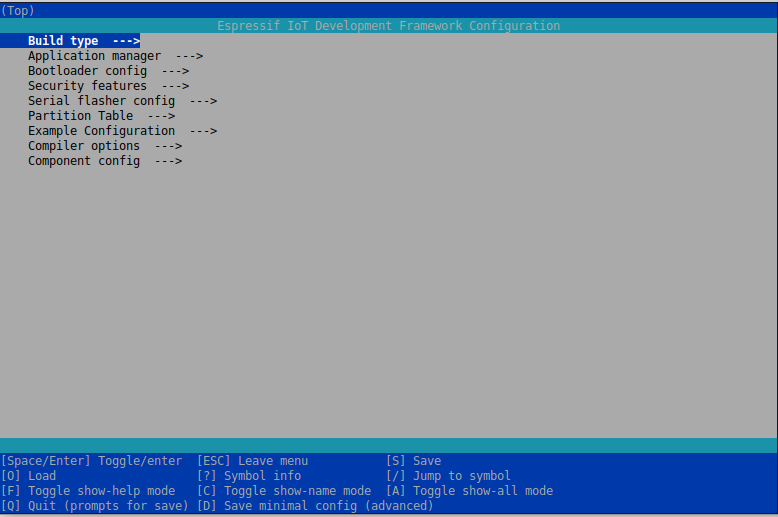
\includegraphics[width=0.7\textwidth]{images/menuConfig.png}
    \caption{Menuconfig window of the project}
    \label{fig:menuConfig} % This is the image label, with which you can refer to the image in any document location.
\end{figure}

Move through the menu using arrow keys end go in \textbf{Example Configuration} to set your personal settings (Wifi connection)
and the peer configuration of WireGuard module (or leave it as it is, to use our configuration) \ref{fig:menuConfig_ex}.

Remember:
\begin{itemize}
    \item \textbf{Wireguard Private Key}: set the private key of the client peer
    \item \textbf{Wireguard remote peer public key}: set the public key of the peer of the server
    \item \textbf{Wireguard local IP address}: set the static IP address of the client peer
    \item \textbf{Wireguard remote peer address}: set the IP address assigned by the router to the server (see NOTE in section \ref{sec:WGprog})
    \item \textbf{Wireguard local/remote peer port}: set the ports for the UDP comunication
    \item \textbf{Target IP address or name}: set the static IP address assigned to the peer server from the server configuration \ref{sec:server}
\end{itemize}

\begin{figure}[H]
    \vspace{0.4cm}
    \centering
    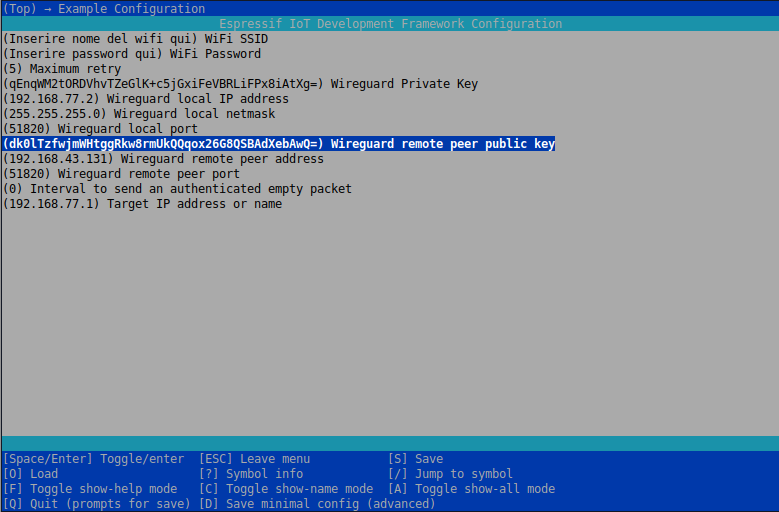
\includegraphics[width=0.7\textwidth]{images/menuConfig_ex.png}
    \caption{Example configuration window in Menuconfig}
    \label{fig:menuConfig_ex} % This is the image label, with which you can refer to the image in any document location.
\end{figure}

\subsection{Build the Project}
Remember to set the environment variable \ref{sec:envSetup} if not done.
Build the project by running:
\begin{lstlisting}
    idf.py build
\end{lstlisting}

This command will compile the application and all ESP-IDF components, then it will generate the bootloader, partition table, and application binaries. 
The first time the command is executed will be slow, then each time a small change is done the build is going to be faster.

\subsection{Connect the Device}
Now connect the ESP32 board to the computer and check under which serial port the board is visible.
\\On Linux the serial ports have \texttt{/dev/tty} naming patterns. So, in order to understand the name of the port assigned to the ESP32
run the command \texttt{ls /dev/tty*} two times, before and after connecting the device and check the difference.
Usually if there are no other USB connections the assigned port should be \texttt{/dev/ttyUSB0}.
Add the User to the dialout group using the following command:
\begin{lstlisting}
    adduser <user_name> dialout
\end{lstlisting} 

\textbf{NOTE}: In case a VM on Windows is used, remember to install the \textit{Silicon Labs CP2102 USB to UART Bridge Controller} driver
on Windows. After that, go under \textbf{Machine $\rightarrowtail$ Settings $\rightarrowtail$ USB} in the VirtualBox Menu bar and add a new USB filter (the plus icon) selecting the correct one

\begin{figure}[H]
    \vspace{0.4cm}
    \centering
    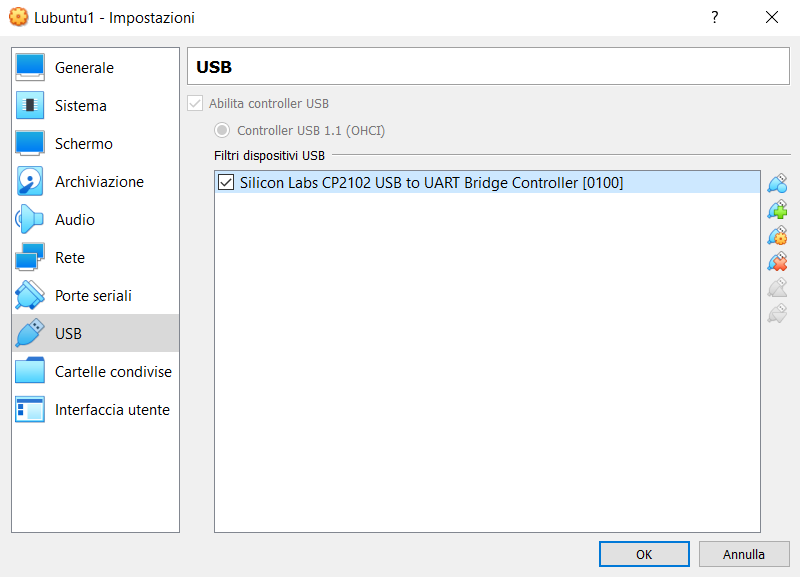
\includegraphics[width=0.75\textwidth]{images/USBex.PNG}
    \caption{Set the USB connection through Oracle VirtualBox VM.}
    \label{fig:USBex} % This is the image label, with which you can refer to the image in any document location.
\end{figure}

\subsection{Flash and Monitor the Device}
Remember to set the environment variable \ref{sec:envSetup} if not done.
Flash the binaries that were built onto the ESP32 board by running:
\begin{lstlisting}
    idf.py -p PORT [-b BAUD] flash
\end{lstlisting}

Replace PORT with the ESP32 board’s serial port name (i.e. /dev/ttyUSB0).
\\To check if the project is indeed running, type the following command that launches the IDF Monitor application:
\begin{lstlisting}
    idf.py -p PORT monitor
\end{lstlisting}

\textbf{Remember}: To exit IDF monitor use the shortcut \texttt{Ctrl+{]}}.

The two commands can be combined in one:
\begin{lstlisting}
    idf.py -p PORT flash monitor
\end{lstlisting}

\subsection{Run the project}
Turn on the Virtual Network Interface on the Server \ref{sec:server}, and listen on a port using Netcat\cite{Netcat} using the following command on the Linux machine running the Server:
\begin{lstlisting}
    nc [-v] -l -p 3333  
\end{lstlisting} 

Or Install "nc for Android" app from the PlayStore \cite{Netcat_android} and use the above command.

\textbf{NOTE}: In case Netcat is note installed on the selected Linux distribution, install with the following command:
\begin{lstlisting}
    sudo apt-get install -y netcat
\end{lstlisting}

After everything is up, turn on the ESP32 (i.e. connecting it to the PC) with the project already flashed.
Other details about the project are explained in \ref{sec:wireguard} 

\section{Start the TCP/IP WG project on FreeRTOS simulator for Linux}\label{sec:WGRtos}
This project is located in the \textbf{Posix\_GCC\_lwip2\_wg} directory.
Here are reported the steps to run the project described in section \ref{sec:addwglinuxsection} starting from the execution of a blinky to download all the needed files.

\subsection{Build a simple "blinky" example}\label{sub:linux_blink}
Follow this procedure to build a simple blinky example from the demo folder of the FreeRTOS distribution.
In order to execute a general project on FreeRTOS simulator for Linux the following steps must be followed. 
\begin{enumerate}
    \item Install some common prerequisite packages: native \textbf{gcc} (the same used to build Linux applications) and \textbf{cmake}.
    \begin{lstlisting}
        sudo apt install gcc cmake
    \end{lstlisting}
    \item Download Freertos: the version used for this project is the one reported here \cite{freertosdownload}.
    \begin{lstlisting}
    git clone https://github.com/FreeRTOS/FreeRTOS.git
    \end{lstlisting}
    \item Make a copy of sample: \texttt{FreeRTOS/Demo/Posix\_GCC}.
    
    This blinky example is made of a software timer (which executes a call-back every 2 seconds) and a thread (infinite loop with a timed wait of 200 ms). Both write a single byte into a message queue on every iteration. Another thread waits for bytes to show up in the queue, recognizes the sender and writes a message for each on \texttt{stdout}.
    \item Build without modification: \texttt{make} inside \texttt{FreeRTOS/Demo/Posix\_GCC}
    
    The project is built using a Makefile: the variable \texttt{SOURCE\_FILES} contains all the source files to be compiled, and the variable \texttt{INCLUDE\_DIRS} is the concatenation of all the include paths to be passed to the compiler command. You may also want to edit \texttt{FREERTOS\_DIR\_REL} at the top of the Makefile if you move the sample to a different folder relative to the FreeRTOS distribution.
    \item run: \texttt{./build/posix\_demo} 
    
    or what you specified in the variables \texttt{BIN} and \texttt{BUILD\_DIR} in the Makefile.
\end{enumerate}

\subsection{Set up TAP}
Set up the TAP on the device, more details here \ref{TapInfo}.
\begin{enumerate}
    \item \texttt{sudo ip tuntap add dev tap1 mode tap user `whoami`} \textit{\# the tap will be called tap1 and be property of the current user}
    \item \texttt{sudo ip link set dev tap1 up}
    \item \texttt{sudo ip addr add 192.168.2.1/24 dev tap1} \textit{\# the computer assigns this address to the interface}
    \item \texttt{export PRECONFIGURED\_TAPIF=tap1} \textit{\# Set the environment variable}
\end{enumerate}

\subsection{Build and run the TCP/IP WG project}
Copy the directory \textbf{Posix\_GCC\_lwip2\_wg} inside \texttt{FreeRTOS/Demo} directory.
In order to set up the WireGuard configuration, change the needed variables inside \texttt{main\_blinky.c} according to the settings of the Client and Server.
Open a Terminal and run Netcat\cite{Netcat} opening the 3333 port:
\begin{lstlisting}
    nc -l -v 3333
\end{lstlisting}

Open a Terminal in the project directory (remember to set up the TAP environment variable) and build:

\begin{lstlisting}
    make
\end{lstlisting}

Execute:
\begin{lstlisting}
    ./build/posix_demo
\end{lstlisting}

\section{Server Configuration}\label{sec:server}
In this section it is analysed how to configure WireGuard on the server side. It is recommended to use a Linux device or an Android device. 
The following instructions are for 3 different types of application:
\begin{itemize}
    \item Linux command line
    \item Windows application
    \item Android application
\end{itemize}

\subsection{Linux server}
In order to setup WireGuard on a Linux environment it is necessary first of all to install the software running
\begin{lstlisting}
sudo apt install wireguard
\end{lstlisting}
Then must be created a private and a public keys for the Wireguard server 
\begin{lstlisting}
wg genkey               # generate private key
echo "<private key>" | wg pubkey    # generate public key
\end{lstlisting}
or to run both commands in the same line and write the keys on two distinct files in the current directory.
\begin{lstlisting} 
wg genkey | tee private.key | wg pubkey > public.key
\end{lstlisting}
At this point remains to decide the IP addresses for the tunnel. A range of IPs could be selected for the interface (i.e. 192.168.77.1/24) that will be the potential values for the available peers.
Now all the required parameters are set and the wg0.conf file could be configured. In this file must be described the interface of the server and the peers (see in section \ref{sec:WGprog} to more details) with code similar to the following one:
\begin{lstlisting}
[Interface]
Address = 192.168.77.1/24
ListenPort = 51820  # default
PrivateKey = {private key}

[Peer]
PublicKey = {public key}
AllowedIPs = 192.168.77.2/32
\end{lstlisting}
The values of the keys are the one generated before and the IPs of the peer must remain in the range of the interface.
Go in the \texttt{/etc/wireguard} and make a new \texttt{wg0.conf} file (must be admin to access the directory).

\begin{lstlisting}
sudo -i
cd /etc/wireguard
nano wg0.conf
\end{lstlisting}

Set up UFW firewall rules to open required ports:

\begin{lstlisting}
sudo ufw allow 51820/udp
\end{lstlisting}

Verify it:

\begin{lstlisting}
sudo ufw status
\end{lstlisting}

Turn the WireGuard service at boot time using the systemctl command, run:
\begin{lstlisting}
sudo systemctl enable wg-quick@wg0
\end{lstlisting}

Start the service, execute:
\begin{lstlisting}
sudo systemctl start wg-quick@wg0
\end{lstlisting}

Get the service status, run:
\begin{lstlisting}
sudo systemctl status wg-quick@wg0
\end{lstlisting}

Verify that interface named wg0 is up and running using the ip command:
\begin{lstlisting}
sudo wg
sudo ip a show wg0
\end{lstlisting}

Done! The WireGuard Server is working.

Remember to use the following commands to turn up or down the Virtual Network Interface
\begin{lstlisting} 
wg-quick up wg0
wg-quick down wg0
\end{lstlisting}

\textbf{NOTE}: In case of using Linux on Oracle VirtualBox VM the network settings of the virtual machine must be adjusted accordingly to server settings.
Go to \textbf{Machine $\rightarrowtail$ Settings $\rightarrowtail$ Network} under Menu bar, make sure it is attached to \texttt{NAT}.
Go under \textbf{Advanced $\rightarrowtail$ Port Forwarding} then add two new forwarding rules with the plus button.
Add a rule for the TCP communication and one for the UDP. An example is shown in \ref{fig:Forwarding} 

\begin{figure}[H]
    \vspace{0.4cm}
    \centering
    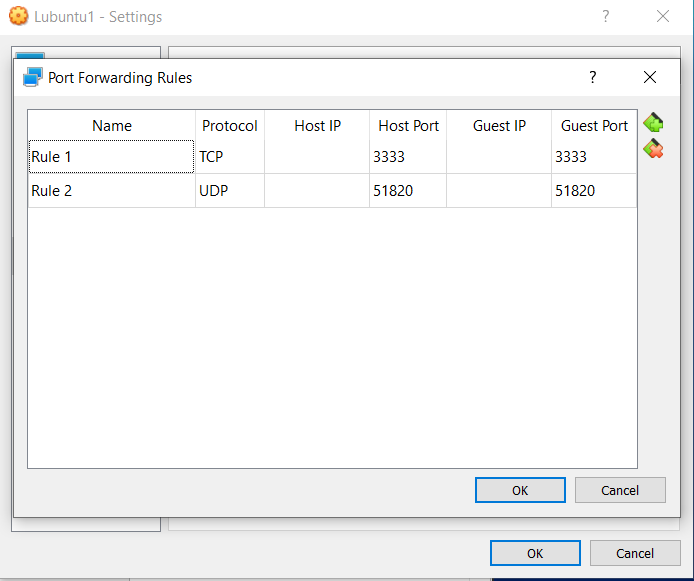
\includegraphics[width=0.75\textwidth]{images/Forwarding.PNG}
    \caption{Forwarding rules for Oracle VirtualBox VM.}
    \label{fig:Forwarding} % This is the image label, with which you can refer to the image in any document location.
\end{figure}

\subsection{Windows server}
On windows it is first of all necessary to install the WireGuard tool from the following link \cite{WireGuardDownload}.
Now you can open the GUI of the tool and create a new tunnel, using the bottom-left button (\ref{fig:wireguard_windows}), where you can create a new empty tunnel or import one from a file. in figure \ref{fig:wireguard_windows_tunnel_settings} there is an example of how to create a new empty tunnel test where there are:
\begin{itemize}
    \item one private interface, that specifies 
    \begin{itemize}
        \item a private key
        \item the listen port of the connection
        \item the address of the network interface
    \end{itemize}
    \item one peer, represented by
    \begin{itemize}
        \item a public key
        \item a range of allowed IPs (in this case only one peer is configured)
    \end{itemize}
\end{itemize}
Once the tunnel is correctly created you can activate it using the activation button, or modify the previous parameters using the bottom-right button.

\begin{figure}[H]
\vspace{0.5cm}
\centering
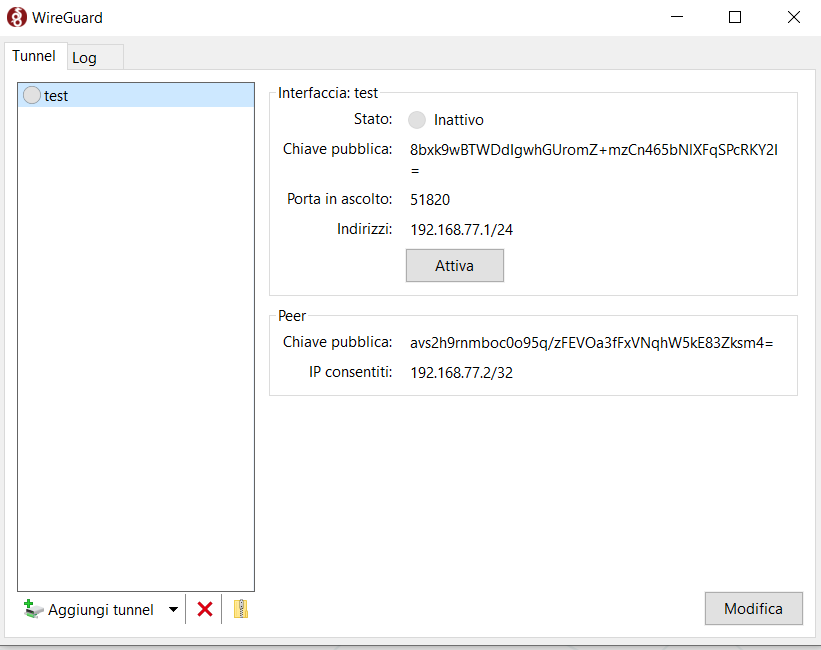
\includegraphics[width=\textwidth/3*2]{images/wireguard_windows.png}
\caption{WireGuard windows application main page.}
\label{fig:wireguard_windows} % This is the image label, with which you can refer to the image in any document location.
\end{figure}

\begin{figure}[H]
\vspace{0.5cm}
\centering
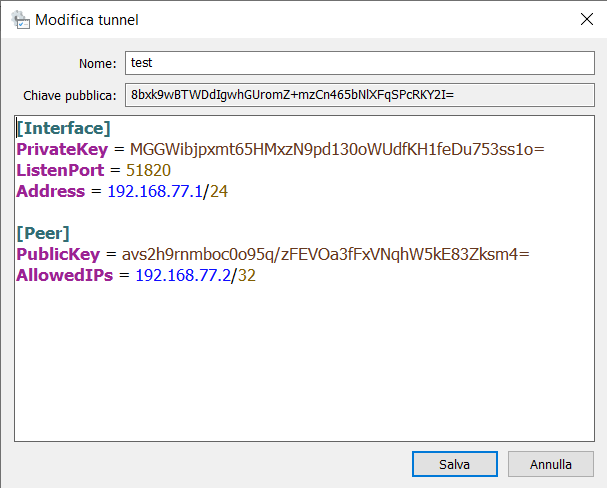
\includegraphics[width=\textwidth/3*2]{images/wireguard_windows_tunnel_settings.png}
\caption{WireGuard windows tunnel settings.}
\label{fig:wireguard_windows_tunnel_settings} % This is the image label, with which you can refer to the image in any document location.
\end{figure}

\subsection{Android server}
Also in this case the first thing to do is to download the application (from the Google Play Store). At the start-up appears the main page (left picture in \ref{fig:android_wireguard_main}), then you can click on the blue button and, selecting for example "build from scratch", you want to create a new tunnel. Now, a page with all the required settings will appear. As explained before must be set the name, the private key and the address for the network interface. Then clicking on "add peer" a peer could be added and could be set also here the public key and the range of IPs. At this point all the setting must be saved pressing the icon in the top-right corner and, using the button shown in the figure on the far right, could be turned on the corresponding tunnel.

\begin{figure}[H]
\vspace{0.5cm}
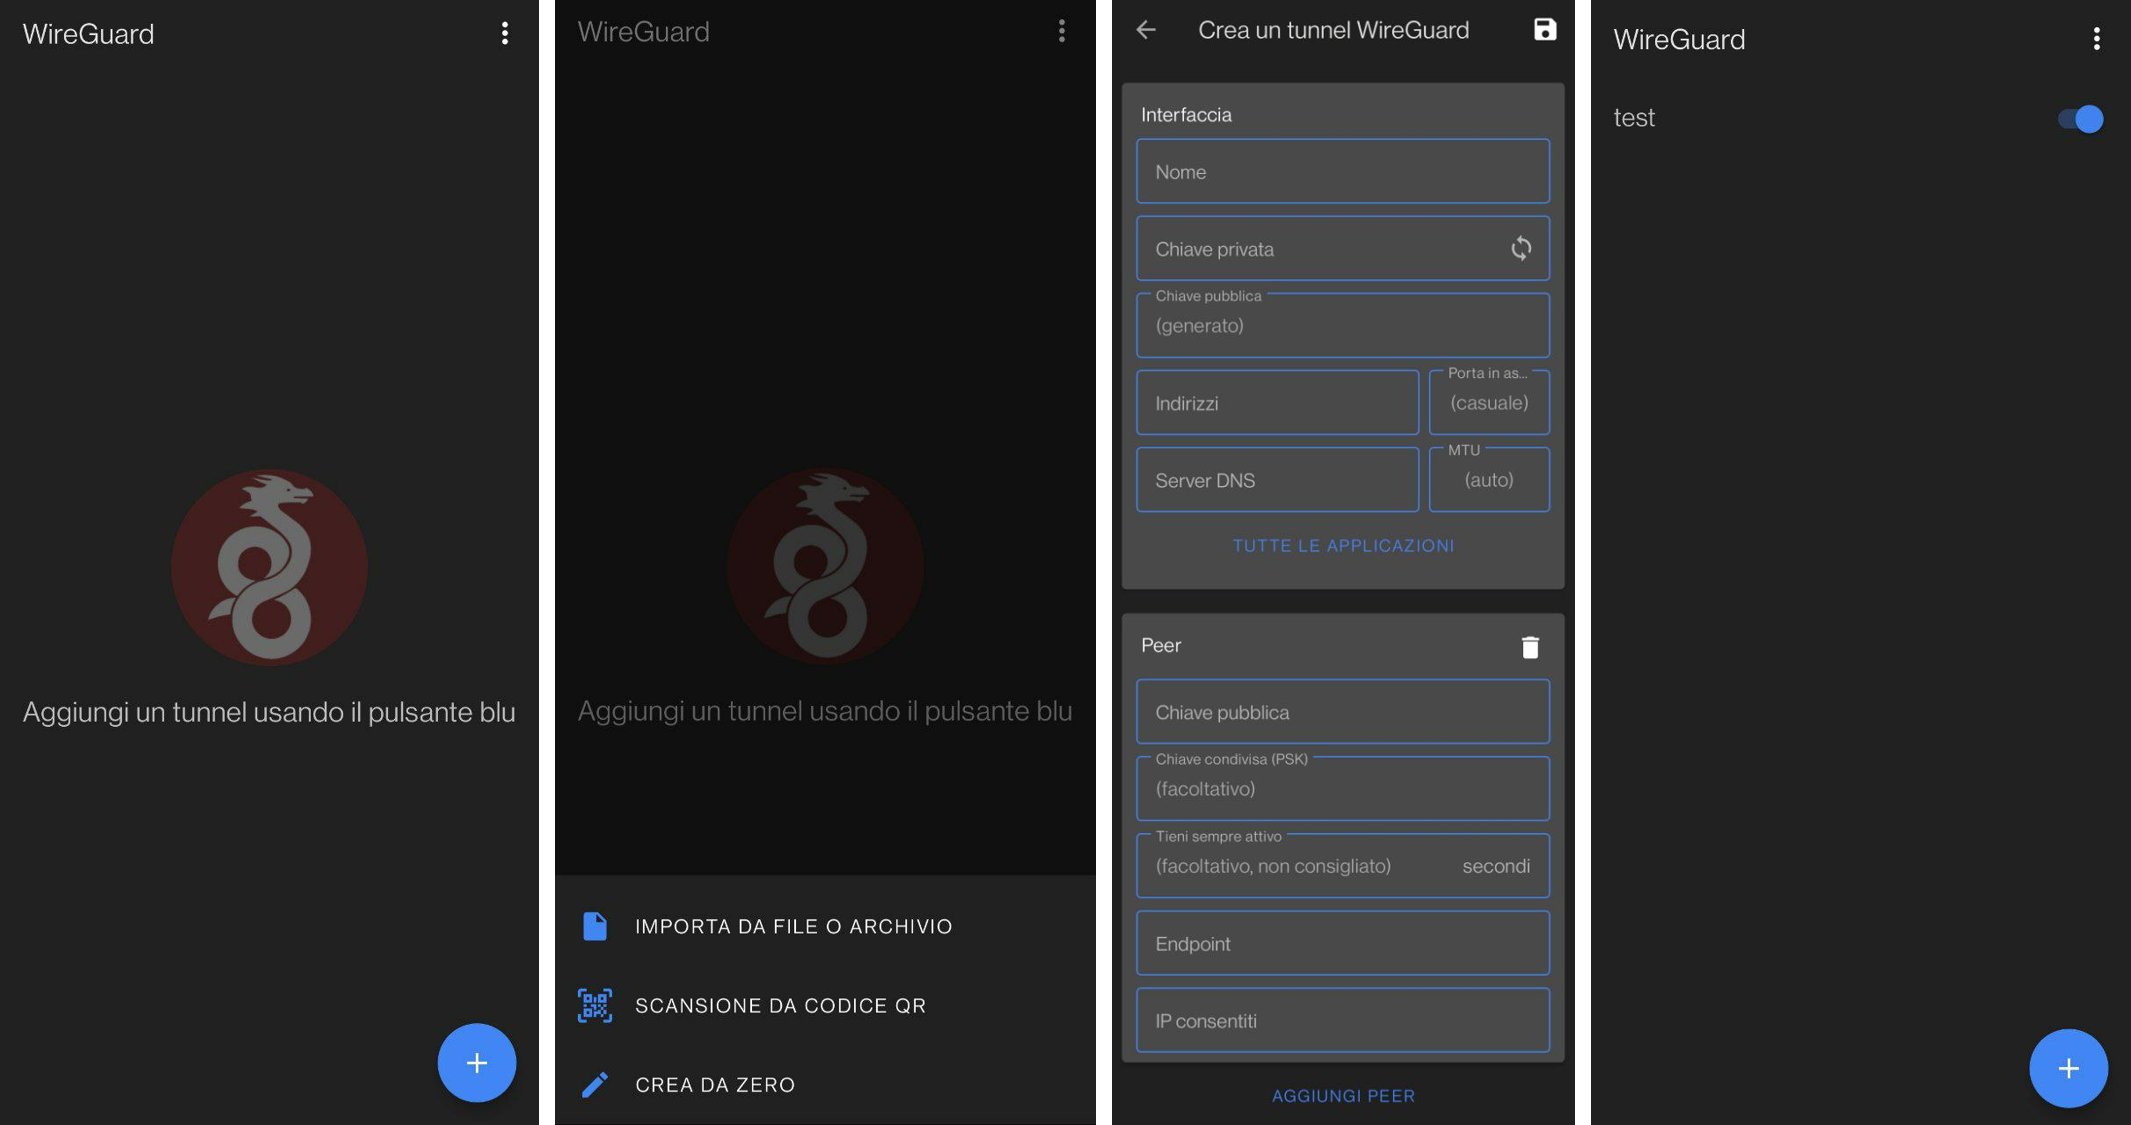
\includegraphics[width=\textwidth]{images/android_server_wg.png}
\caption{WireGuard android application.}
\label{fig:android_wireguard_main} % This is the image label, with which you can refer to the image in any document location.
\end{figure}


